\documentclass[11pt,a4paper]{article}
\usepackage[T1]{fontenc}
\usepackage{lmodern}
\usepackage{amssymb,amsmath}
\usepackage{ifxetex,ifluatex}
\usepackage{fixltx2e} % provides \textsubscript
% use upquote if available, for straight quotes in verbatim environments
% \usepackage[sc,osf]{mathpazo}
\usepackage{helvet}
\renewcommand{\familydefault}{\sfdefault}
% \usepackage{crimson}
\IfFileExists{upquote.sty}{\usepackage{upquote}}{}
% \ifnum 0\ifxetex 1\fi\ifluatex 1\fi=0 % if pdftex
%   \usepackage[utf8]{inputenc}
% % \else % if luatex or xelatex
%   \ifxetex
%     \usepackage{mathspec}
%     \usepackage{xltxtra,xunicode}
%   \else
%     \usepackage{fontspec}
%   \fi
%   \defaultfontfeatures{Mapping=tex-text,Scale=MatchLowercase}
%   \newcommand{\euro}{€}
% % % % % \fi
% use microtype if available
\IfFileExists{microtype.sty}{\usepackage{microtype}}{}
% % % \usepackage{biblatex}
% 
\usepackage[backend=biber,style=authoryear-comp,natbib,sortcites=none,autopunct=true]{biblatex}
\renewcommand*{\nameyeardelim}{\addspace}

% 
\usepackage{longtable,booktabs}



\usepackage{graphicx}
% Redefine \includegraphics so that, unless explicit options are
% given, the image width will not exceed the width of the page.
% Images get their normal width if they fit onto the page, but
% are scaled down if they would overflow the margins.
\makeatletter
\def\ScaleIfNeeded{%
  \ifdim\Gin@nat@width>\linewidth
    \linewidth
  \else
    \Gin@nat@width
  \fi
}
\makeatother
\let\Oldincludegraphics\includegraphics
{%
 \catcode`\@=11\relax%
 \gdef\includegraphics{\@ifnextchar[{\Oldincludegraphics}{\Oldincludegraphics[width=\ScaleIfNeeded]}}%
}%

% \ifxetex
%   \usepackage[setpagesize=false, % page size defined by xetex
%               unicode=false, % unicode breaks when used with xetex
%               xetex]{hyperref}
% \else
%   \usepackage[unicode=true]{hyperref}
% \fi

\usepackage[colorlinks=true, urlcolor=blue, linkcolor=black, citecolor=blue, pdfauthor={Adam La Caze}]{hyperref}



% \urlstyle{same}  % don't use monospace font for urls

\providecommand{\tightlist}{%
  \setlength{\itemsep}{0pt}\setlength{\parskip}{0pt}}

\setlength{\parindent}{0pt}
\setlength{\parskip}{6pt plus 2pt minus 1pt}
\linespread{1.05}

\setlength{\emergencystretch}{3em}  % prevent overfull lines
\setcounter{secnumdepth}{5}

\title{Pharmacist responsibilities when selling complementary medicines}
\author{}
\date{}
\usepackage{array}

\def\UrlBreaks{\do\/\do-\do?}

\newcommand{\vers}{v0.1 \hfill \today}

\newcommand\T{\rule{0pt}{2.6ex}}       % Top strut
\newcommand\B{\rule[-1.2ex]{0pt}{0pt}} % Bottom struct

\addbibresource{library.bib} %only if using biblatex

\begin{document}
\maketitle

\begin{tabular}{ll} Adam La Caze & Senior Lecturer\tabularnewline
& School of Pharmacy\tabularnewline
& The University of Queensland\tabularnewline
& a.lacaze@uq.edu.au\tabularnewline[10pt] Amber Salman Popattia & School of Pharmacy\tabularnewline
& The University of Queensland\tabularnewline
& amber.salmanpopattia@uqconnect.edu.au\tabularnewline[10pt] Laetitia Hattingh & Adjunct Associate Professor\tabularnewline
& School of Pharmacy and Pharmacology\tabularnewline
& Griffith University\tabularnewline
& L.Hattingh@griffith.edu.au\tabularnewline
\end{tabular}

\vfill
This is a draft report for the project \emph{Evaluating the
acceptability and feasibility of an ethical framework for the sale of
complementary medicines in community pharmacy} funded by an APSA
Research Grant 2019.

\bigskip
\textbf{Version}:
\href{https://github.com/alacaze/cmethics_apsa}{62ecc18} \hfill 28
January, 2020

\newpage 

\tableofcontents

\newpage

\section{Synopsis}\label{synopsis}

Many consumers choose to use complementary medicines and frequently
purchase their complementary medicines from community pharmacy.
Pharmacists tend to vary in their approach to the sale of complementary
medicines and recent media reports suggest that some pharmacies are
failing to meet community expectations regarding the advice they
provide. There is a need for clearer guidance for pharmacists regarding
their responsibilities when selling complementary medicines. The
investigators have developed an ethical framework for the sale of
complementary medicines in community pharmacy. This project evaluated
the acceptability and feasibility of implementing an ethical framework
for the sale of complementary medicines in community pharmacy developed
by the investigators. Seventeen community pharmacists participated in
four focus groups and six individual interviews. There was good
representation among participants in terms of gender, years of practice,
pharmacy location and script volume.

\section{Background}\label{background}

This project seeks to contribute to pharmacy practice by developing
clear guidance to pharmacists regarding their responsibilities when
selling complementary medicines. Complementary medicines are a \$4.9
billion dollar industry in Australia, 41\% of which is sold through
pharmacies \autocite{ComplementaryMedicinesAustralia2018}. Consumers
purchase complementary medicines from pharmacies due to a trust in the
quality of the products and the availability of advice.{[}REF{]} There
is clear recognition that pharmacists should (i) support consumer choice
and (ii) provide advice that is informed by evidence
\autocites{InternationalPharmaceuticalFederation2014}{PSA2017}. There
is, however, very little guidance on what to do when these two
principles conflict \autocite{SalmanPopattia2018}. The conflict arises
because many complementary medicines lack rigorous evidence of
effectiveness and yet can cause harm through adverse effects, drug
interactions and delayed treatment \autocites{Myers2004}{Izzo2009}. In
the absence of evidence of benefit, evidence-based guidance suggests
that pharmacists should avoid selling complementary medicines
\autocite{Ernst1996}. Recent reports suggest that pharmacists are
failing to meet community expectations regarding the advice they provide
on complementary medicines
\autocites{Bray2017}{Thompson2017}{Arnold2016}[.][]{King2017}

\textcite{SalmanPopattia2018} identify several gaps in the literature
examining the responsibilities of pharmacists selling complementary
medicines. The most striking of these is the lack of specific guidance
for pharmacists on the sale of complementary medicines. The expectations
of pharmacists and consumers regarding the sale of complementary
medicines are well described
\autocites{Iyer2016a}{Tran:2013kh}{Kanjanarach2011}. To the extent that
ethical considerations are discussed in this literature, the conflict
between supporting consumer choice, evidence-based practice and business
considerations are frequently identified but never resolved. Part of the
problem is the lack of an explicit ethical theory to guide
decision-making. While the `four principles approach' of bioethical
principlism is implicit in many discussions, the version that is
employed focuses on `ethics first-aid': the \emph{identification} of
ethical conflicts rather than resolution of the conflict
\autocites{Beauchamp2012}{Pullman2005}

The problems associated with the lack of specific guidance for
pharmacist responsibilities when selling complementary medicines is
highlighted by the current \emph{Code of ethics for pharmacists}
\autocite{PSA2017}. While the code provides the advice to support
consumer choice and to practice in accordance with evidence, it also
provides the directive that pharmacists will ``only purchase, supply or
promote any medicine, complementary medicine, herbal remedy or other
healthcare product where there is credible evidence of efficacy and the
benefit of use outweighs the risk''. This directive is in contrast with
current practice in which complementary medicines that lack credible
evidence of efficacy are frequently purchased and supplied. There is no
attempt to reconcile this disparity in the professional or academic
literature---no explicit argument for the directive provided in the
code, nor a counter-argument defending the routine sale of complementary
medicines that lack evidence of efficacy in community pharmacy.

Salmon Popattia and La Caze have developed an ethical framework that
provides specific guidance to pharmacists regarding their
responsibilities when selling complementary medicines. An overview of
the framework is provided below.

\section{A framework for pharmacist responsibilities when selling
complementary
medicines}\label{a-framework-for-pharmacist-responsibilities-when-selling-complementary-medicines}

There are three components to the framework: principle-based ethics
provides the theoretical foundations, a \emph{public health argument}
provides \emph{prima facie} support for the sale of complementary
medicines in community pharmacy, and specific responsibilities are
provided that ensure that pharmacists meet their obligations to the
public when selling complementary medicines.

\subsection{Principle-based ethics}\label{principle-based-ethics}

Principle-based ethics, and more specifically, the `four principles
approach' to bioethics advocated by \textcite{Beauchamp2012}, is
frequently employed in bioethics and professional ethics in health care.
The four principles are \emph{respect for autonomy},
\emph{beneficience}, \emph{non-maleficence}, and \emph{justice}. The
theory provides resources for further specifying these general
principles when they conflict in particular contexts. The
approach---using \emph{reflective equilibrium} and
\emph{specification}---provides a framework for responding to ethical
challenges by explicitly weighing up and resolving conflicts in general
principles based on salient details within the context {[}REF{]}.

The specific responsibilities provided by the framework were developed
by weighing up mid-level principles such as the need for pharmacists to
provide evidence-based care as well as to respect the health beliefs and
preferences of consumers. These mid-level principles can be derived from
more general guiding principles, such as ensuring positive health
outcomes in consumers (beneficence and non-maleficence) and respecting
autonomy. The framework seeks to resolve the conflicts that arise in
these principles in relation to pharmacists selling complementary
medicines.

\subsection{Public health argument}\label{public-health-argument}

The second component of the framework is a public health argument for
pharmacists selling complementary medicines. This argument is driven by
two key points. First, complementary medicines are regulated in
Australia (and most regions in the world) as being sufficiently safe for
self-care. Most complementary medicines available in community pharmacy
are \emph{listed} on the Australian Register of Therapeutic Goods
\autocite{TGA2019_listed}. This means that the complementary medicine
contains items that are on a list of low-risk ingredients, is
manufactured according to the principles of Good Manufacturing Practice,
and the only claims made regarding therapeutic use relate to the
maintenance and enhancement of health for non-serious, self-limiting
conditions. Listed medicines are available from a wide range of outlets,
including pharmacies, health food stores, and supermarkets. Many
consumers choose to use complementary medicines and are likely to
continue to do so even if they were not available in community
pharmacies.

Second, pharmacists are a highly accessible health professional with the
training and skills to provide guidance on the appropriate use of
complementary medicines. In particular, pharmacists have excellent
skills in being able to identify and resolve potential drug interactions
and to provide guidance regarding actual or potential adverse reactions.
Pharmacists tend to focus on this role in relation to complementary
medicines and consumers frequently identify this support as one of the
drivers for purchasing complementary medicines from community pharmacies
\autocites{Olatunde2010}{Kanjanarach2011}.

The combination of these points provides a \emph{prima facie} argument
in support of the sale of complementary medicines in community pharmacy.
However, for the argument to be compelling pharmacists and pharmacy
support staff need to be proactive in providing evidence-based advice to
consumers. This is not always the case. Some pharmacists are hesitant to
discuss complementary medicines with consumers, and some provide
inaccurate or misleading information regarding the likely benefits of
complementary medicines
\autocites{SalmanPopattia2018}{Arnold2016}{Bray2017}. The specific
responsibilities of pharmacists when selling complementary medicines
outlined below seek to address these issues. The framework identifies
the responsibilities that pharmacists must meet in order to make a
positive contribution to health outcomes by selling complementary
medicines.

\subsection{Specific responsibilities}\label{specific-responsibilities}

The key responsibilities outlined by the framework are provided in
Table~\ref{responsibilities}. The responsibilities overlap in some
respects, but each articulates a specific responsibility for pharmacists
working in a community pharmacy and managing staff in relation to
complementary medicines. The framework makes a distinction between
pharmacy staff making an \emph{explicit recommendation} to take a
complementary medicine, and selling complementary medicines without an
explicit recommendation. The framework suggests that
\emph{recommendations} for a complementary medicine must be consistent
with current best evidence, and all \emph{sales} of a complementary
medicine should be accompanied with an \emph{offer} of advice from a
pharmacist. If consumers take up that offer of advice, a pharmacist must
be available to provide that advice and to provide sufficient
information to the consumer such that they can make an informed decision
with regard to the purchase of the complementary medicine. Since some
consumers might refuse the offer of advice from a pharmacy, it is the
responsibility of the pharmacist to have procedures in place to identify
and act if a consumer is at significant risk of harm from complementary
medicines. Further advice regarding the responsibilities outlined in the
framework are available in Appendix A.

\begin{table}
\centering
\begin{tabular}{p{0.8\linewidth}}
\hline\T
1. Pharmacists should provide evidence-based recommendations to the consumers regarding complementary medicines\\[10pt]
2. Pharmacists should train all staff in a pharmacy and ensure that they provide evidence-based recommendations regarding complementary medicines and seek advice of a pharmacist when required\\[10pt]
3. When providing advice, pharmacists should provide sufficient information for consumers to make informed decisions regarding complementary medicines\\[10pt]
4. Pharmacists should setup the pharmacy so that consumers are provided an offer of advice from a pharmacist and pharmacists should be available to provide that advice\\[10pt]
5. Pharmacists must be vigilant for possible harms related to complementary medicines and intervene if risk of harm is significant\B\\
\hline
\end{tabular}
\caption{The key responsibilities of pharmacists selling complementary medicines}
\label{responsibilities}
\end{table}


\section{Aim}\label{aim}

The \textbf{specific aim} of this project is to evaluate the
acceptability and feasibility of the proposed ethical framework for the
sale of complementary medicines in community pharmacy. The project also
sought to identify any barriers to the acceptance and/or implementation
of the framework in community pharmacy.

\section{Methods}\label{methods}

Australian community pharmacists were invited to participate in online
workshops via a videoconferencing platform in September and October
2019. Pharmacists were be recruited using social media, professional
organisations, and communication through the professional networks of
key community pharmacy banner groups. If necessary, purposive sampling
was to be employed to ensure that the age and gender distribution of
participants reflects the workforce and that participants are recruited
with different levels of experience and from different practice
environments (small independent pharmacies, large chains, and
discount-oriented pharmacies).

The workshops employed focus group methods to engage participants in
discussion regarding the sale of complementary medicines in community
pharmacies. Focus groups provide an opportunity to investigate complex
behaviours and motivations, to learn more about the degree of consensus
on a topic, and to gain feedback regarding new ideas
\autocites{Basch1987}{Knodel1993}. They are especially helpful to
understand group norms, meanings and processes \autocite{BarbourFG2011}.
Workshops were offered inside and outside of usual business hours using
video-conferencing software, Zoom. Conducting focus groups via
video-conference provided an opportunity to recruit participants from a
large geographical area. A number of strategies were employed to support
the success of conducting the focus group in an online environment,
these included seeking to arrange groups of 4--6 participants (limiting
larger groups), enabling video feeds and offering alternatives for those
with lower internet speeds \autocite{Gaiser2017}.

Participants received information about the framework prior to the
workshop and were asked to complete a short pre-workshop survey. The
objectives of the workshops were (i) to examine the range of views
community pharmacists have regarding their responsibilities when selling
complementary medicines; (ii) to assess perceived appropriateness and
feasibility of the developed ethical framework; (iii) to identify
organisational, professional and personal barriers to the acceptance
and/or implementation of the ethical framework, and (iv) to aid the
development of specific guidance for pharmacists in applying the ethical
framework. Discussion topics explored the context in which pharmacists
provide advice on complementary medicines within community pharmacy, and
the acceptability and feasibility of the proposed ethical framework. The
semi-structured interviews conducted with participants unable to join a
workshop followed the same structure.

All focus groups and interviews were conducted by AL. It was made clear
from the start of each focus group and interview that the objective of
the discussion was to understand the participants views and how they
varied. Participants were encouraged to share diverging views and to
debate topics in a respectful manner. The facilitator did not share
views during the focus groups or interviews. ASP was an observer for
most of the focus groups and interviews. AL and ASP debriefed
immediately following each focus group and interview and prepared the
summary that was sent to participants for comment.

The workshops and interviews were video and audio recorded. Focus groups
and interviews were transcribed verbatim. The transcripts were analysed
using the thematic analysis methods described by Braun and Clarke
\autocite*{Braun2016}. An inductive approach to coding was employed, and
themes were developed with a focus on addressing the research questions
in the study. Two investigators, AL and ASP, familiarized themselves
with the data and developed an initial coding scheme. This was refined
through discussion early in the analysis and then used to code the focus
groups and interviews. AL and ASP then identified and refine themes
individually first, and then as a group that included LH.

All three investigators have experience in pharmacy ethics. AL has
experience in qualitative research, facilitation of online groups and
research and teaching in ethical reasoning and decision-making in
pharmacy practice. ASP has a background in nursing and bioethics and
developed the ethical framework as part of PhD. LH has experience in
health law and ethics and qualitative research. LH was involved in
development of the Pharmaceutical Society of Australia \emph{Code of
ethics for pharmacists}.

\section{Results}\label{results}

Seventeen community pharmacists participated in 4 workshops and 6
individual interviews. The workshops contained 2--4 participants and
went from 29 to 68 minutes in duration (median duration 42.5 minutes).
The duration of the interviews ranged from 17 to 34 minutes (median 21
minutes). Demographic features of the participants are provided in Table
2. Participants varied in terms of gender, years of practice and type of
pharmacy and typical script volume. More than a third of participants
worked in a regional or rural location.

\begin{table}[htb]
\centering
\begin{tabular}{llc}
\hline
\multicolumn{2}{l}{\textbf{Demographics}}                                                                                                                   & \textbf{N}  \T\B\\
\hline
Gender            & Male                                                                                                                           & 9  \T\\
                  & Female                                                                                                                         & 8  \\
Years of practice & 1--5                                                                                                                            & 5  \\
                  & 6--10                                                                                                                           & 6  \\
                  & 11--20                                                                                                                          & 3  \\
                  & 20+                                                                                                                            & 3  \\
Type of pharmacy  & Large shopping centre                                                                                                          & 5  \\
                  & Small local                                                                                                                    & 6  \\
                  & Extended hours                                                                                                                 & 3  \\
                  & Discount                                                                                                                       & 3  \\
Location          & Urban area                                                                                              & 11 \\
                  & Regional area  & 5  \\
                  & Rural area              & 1  \\
Script volume     & 0--50 prescriptions                                                                                                            & 1  \\
                  & 50--100 prescriptions                                                                                                          & 4  \\
                  & 100--200 prescriptions                                                                                                         & 1  \\
                  & 200--300 prescriptions                                                                                                         & 3  \\
                  & 300+ prescriptions                                                                                                             & 8\B\\
\hline
\end{tabular}
\caption{Demographic features of the participants}
\end{table}

The presurvey questions provide a snapshot of the participants views
about complementary medicines in terms of their day-to-day practice.
Most participants agreed with statements regarding providing advice to
consumers about complementary medicines as being part of their role, and
feeling positive about the advice they give to consumers regarding
complementary medicines. Participants were less likely to agree with
statements regarding their possession of the necessary knowledge and
skills in relation to complementary medicines, and a statement regarding
possessing the necessary time and resources to help consumers with
complementary medicines.

\begin{figure}
\centering
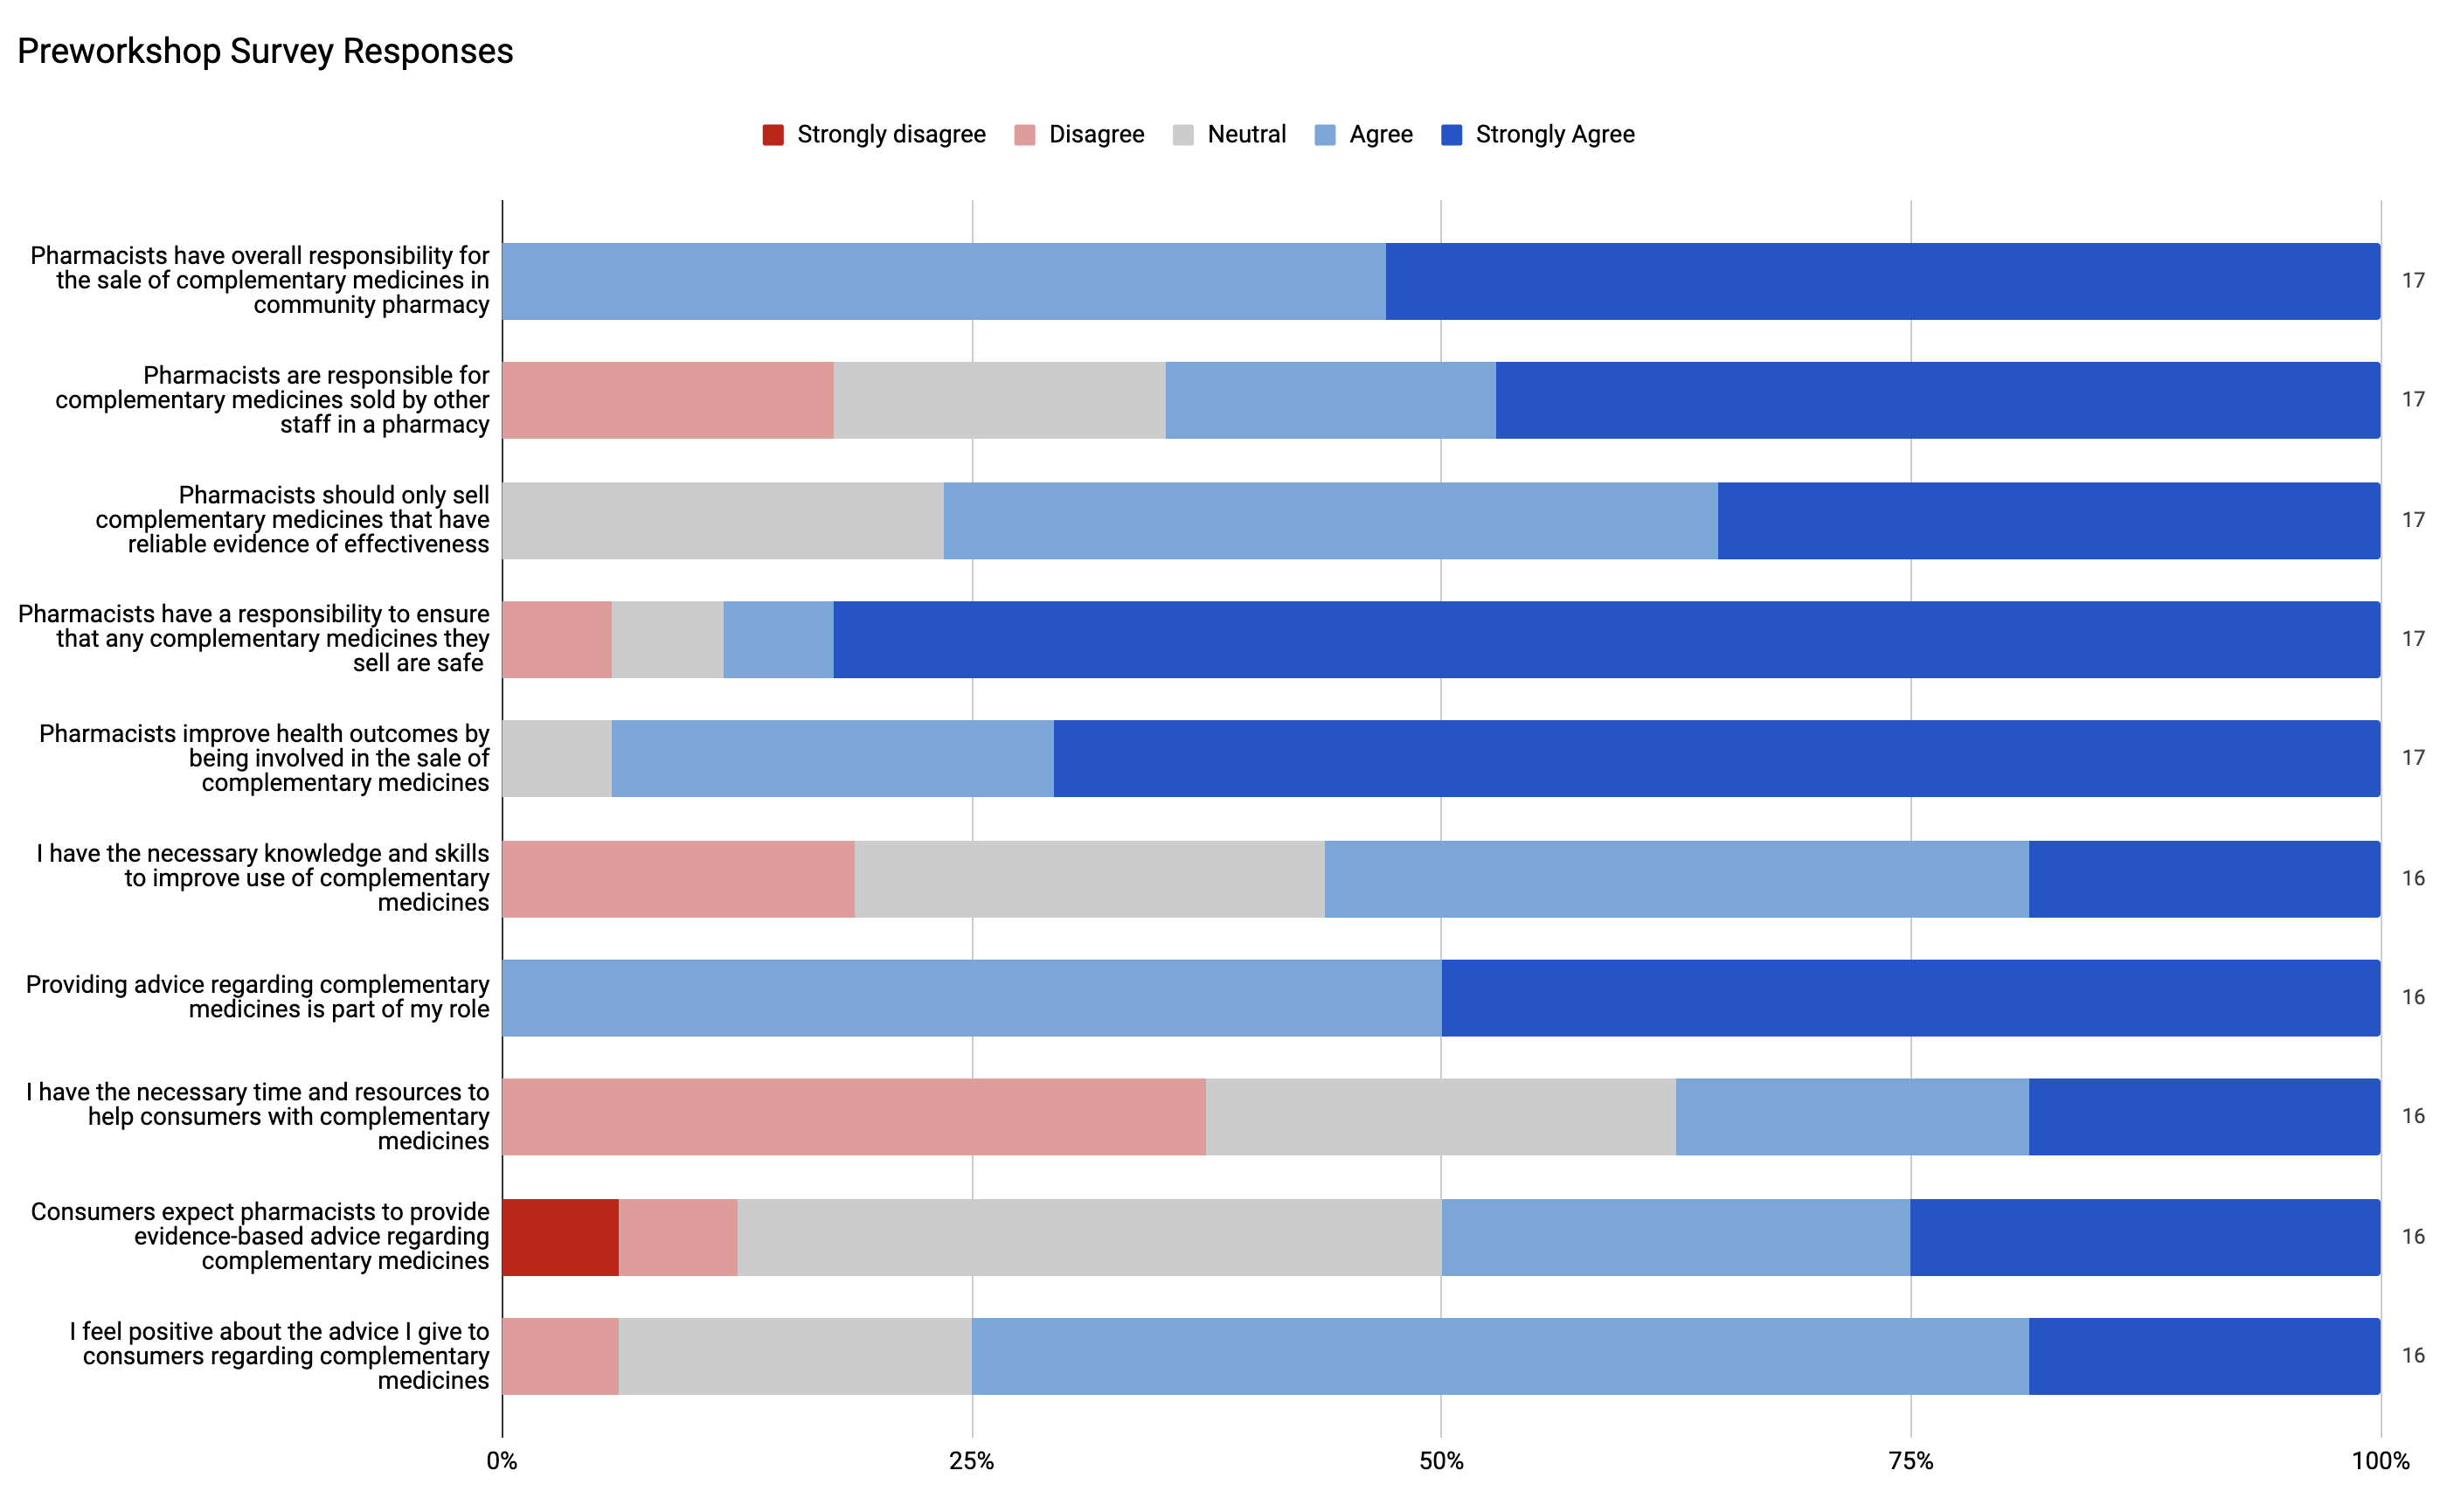
\includegraphics{fig_tab/presurvey.png}
\caption{Results of the presurvey. Statements are ordered by the
percentage of agreement of the participants.}
\end{figure}

\subsection{Key themes}\label{key-themes}

The focus groups provided rich information on how pharmacists approached
their practice in relation to complementary medicines, their perceptions
of the framework and their views regarding the facilitators and barriers
to implementing the framework in practice. Thematic saturation occurred
after 3 focus groups and 4 interviews, additional focus groups and
interviews helped to explore and confirm key findings. Three main themes
emerged from the focus groups and interviews. These themes are
summarised in Table 3. The first two themes represent spectra on which
participants differed: \emph{Approach to complementary medicines
(proactive--reactive)} and \emph{Approach to evidence}. The third theme,
\emph{Navigating practice in a retail environment}, represents the
recognition from all participants that community pharmacy is in a retail
environment and decisions regarding professional practice have resource
and other financial implications.

\begin{table}[tbh]
\centering
\begin{tabular}{>{\raggedright}p{0.5\linewidth}l}
\hline
\textbf{Theme}                               & \textbf{Relevance}\T\B\\
\hline
Approach to complementary medicines                 & Context, Feasibility       \T\\[21pt]
Approach to evidence  & Context, Acceptability     \\[10pt]
Navigating practice in a retail environment  & Acceptability, Feasibility\B\\
\hline
\end{tabular}
\caption{Key themes from the focus groups and interviews and the relevance these themes had on the context of complementary medicine sales in community pharmacy and the acceptability and feasibility of the proposed framework}
\end{table}

The ways in which participants \emph{approached complementary
medicines}, \emph{approached evidence}, and \emph{navigated practice in
a retail environment} inform how they viewed their responsibilities in
relation to complementary medicines within the context of community
pharmacy practice and their views on the acceptability and feasibility
of the proposed framework. Each of these themes are briefly introduced
below. Subsequent sections provide further discussion regarding how
participant responses within these themes addresses the objectives of
the project. Understanding these themes, and the ways in which
participants varied within the themes provide insight into the
\emph{context} (Section \ref{context}) of community pharmacy practice in
relation to complementary medicines, and the \emph{acceptability} and
\emph{feasibility} of the framework as perceived by the participants
(Section \ref{acceptability} and \ref{feasibility}).

\subsubsection{Approach to complementary
medicines}\label{approach-to-complementary-medicines}

A number of participants described their practice in terms of a
proactive approach to complementary medicines. These participants tended
to initiate discussion regarding complementary medicines with consumers
and see an important role for pharmacists in being active in relation to
complementary medicines.

\begin{quote}
Pharmacists are becoming more involved than before. People are trusting
pharmacists more. They always check their complementary medicine. I
think, from what I remember five years ago, people were just picking it
up. They were thinking that, ``That's just a supplement,'' but I think
the awareness is more than before among people. So they always come and
ask, ``Oh, is this one safe?'' or, ``What should I take?'' I think now,
lots of pharmacists are always checking things for them.
(D1P1)\footnote{Workshops and interviews are labelled as ``Discussions''
  and numbered in order. ``Participants'' are also allocated a number in
  order. ``D1P1'' refers to Discussion 1, Participant 1.}
\end{quote}

Some participants worked in community pharmacies set-up to provide
specialist advice on complementary medicines, including the use of
practitioner-lines.

\begin{quote}
I work in a small community pharmacy. I probably consider myself a
integrated pharmacist. We have complementary medicines in three
different areas similar to the rest of your medicines, like S2s, S3s. So
we've got some out in the front shop, which I consider your
{[}day-to-day{]} vitamins, like your supermarket lines. They're more
lines that are more for patients to choose and that sort of thing if
they want to self-select. If they go for advice from a pharmacist or
staff member, we'd probably go for something a bit better quality. So
we've got some in the S2 section which are, I guess, better quality
practitioner ranges. And then we've got your other ones in your S3 areas
which are ranges that do require a consult or a prescription. So a lot
of them are prescribed by some of our doctors as well. (D7P13)
\end{quote}

By contrast, other participants adopted a reactive approach to
complementary medicines. These participants indicated that they are less
likely to initiate discussion of complementary medicines with consumers,
and were more likely to express a lack of confidence in complementary
medicines. Participants expressing these views tended to rely more
heavily on support staff in this area.

\begin{quote}
I suppose it's not as big a focus in my professional practice\ldots{}. I
think it's probably because of lack of knowledge, to be honest, and
confidence, where you feel a lot more secure at the back counter or in a
dispensary than you do out in the vitamin section. (D5P8)
\end{quote}

For some participants, a reactive role towards complementary medicines
was seen as a consequence of the lack of evidence for the effectiveness
of many of these medicines.

\begin{quote}
Yeah. I think at the moment, I don't think we have much role to play in
selling or providing any counselling for complementary medicine because
first, working in community pharmacy, our main role is actually just
dispensing. And then pharmacies, I think, we should follow more like
evidence-based medicine practise\ldots{}. All this supplementary of
complementary medicine and all, they're not evidence-based. (D5P6)
\end{quote}

\subsubsection{Approach to evidence}\label{approach-to-evidence}

Participants also varied in their approach to evidence. Most, if not
all, participants explicitly endorsed ``evidence-based practice'' in
relation to complementary medicines, but what participants took this to
mean and how it related to their day-to-day practice tended to differ.

Many participants described their practice in a way that is consistent
with evidence-based practice while also recognising some of the
challenges.

\begin{quote}
{[}W{]}e shouldn't just be selling things because someone \ldots{} says,
``Oh, this turmeric is great for the sake of curing cancer.'' I think
there has to be some level of evidence\ldots{} And it's hard in certain
conditions because you're just never going to have the trials. (D4P5)
\end{quote}

A number of participants felt there should be a greater emphasis on
evidence-based practice in relation to complementary medicines.

\begin{quote}
If we, I think, perhaps as an industry, move towards more-- well, what
is the evidence? Do I feel that your needs will be met by what I'm
recommending today? Is there evidence to support what it says on the
label, or what it says in the marketing material? And if not, then maybe
we, as an industry, could push the emphasis of companies bringing things
to market, being more about actual evidence. More money going into these
studies of N equals 50. (D5P9)
\end{quote}

Some participants, however, expressed views inconsistent with
evidence-based practice. These participants put significantly more
weight into anecdotal reports and placebo effects as providing evidence
for the effectiveness of complementary medicines. In response to the
explicit PSA guidance to only sell complementary medicines that are
efficacious, one participant felt that placebo effects were sufficient
to meet this standard.

\begin{quote}
So how I would actually interpret {[}the PSA guidance{]}, and this is
where placebo effects comes in. So hey, if it's not doing them any harm
and they think it's better for them and they're going on in their life
and happy days, you just let them go. (D5P7)
\end{quote}

Other participants put a lot of value into anecdotal experience.

\begin{quote}
So I see a lot of people really---a lot of people want to use it. I've
talked to a lot of customers, and they do feel the result. Every time
they come back, I always ask, ``Is this working for you?'' And a lot of
times, they say, ``Yes, I know it's working because when my bottle ran
out, I started feeling it.'' So then they came back to get a new bottle.
So regarding your first question where you say, ``What's our perspective
regarding purchase of natural medications?'' I think they really work. I
think they work depending what the situation is. There are some
situations where you obviously need something more potent. But even in
those situations, I think there's always a place for natural medication,
either as a stand-alone treatment or in combination. This is just based
on what I've seen, not just what I think, what I've seen from what
people say. (D9P16)
\end{quote}

Participants tended to vary according to their approach to complementary
medicines and approach to evidence independently. Different participants
expressed each of the following views: ``proactive and evidence-based'',
``reactive and evidence-based'', ``proactive and less evidence-based''
and ``reactive and less evidence-based'' (see Figure~\ref{context3}).
Here, for example, is one of the participants suggesting that most
pharmacists they knew were ``reactive and evidence-based''

\begin{quote}
I would think in the most part people are very reactive. I don't know
that people would proactively engage in conversations a lot in my
experience. But I think if they were asked, then they would provide
evidence-based information to the best of their knowledge. (D6P10)
\end{quote}

Where participants exist on these spectra informed their response to a
variety of topics regarding the sale of complementary medicines in
community pharmacy, including the role of naturopaths, the availability
and confidence the participant had with regard to information resources,
practitioner-only products and the proposed framework.

\begin{figure}
\centering
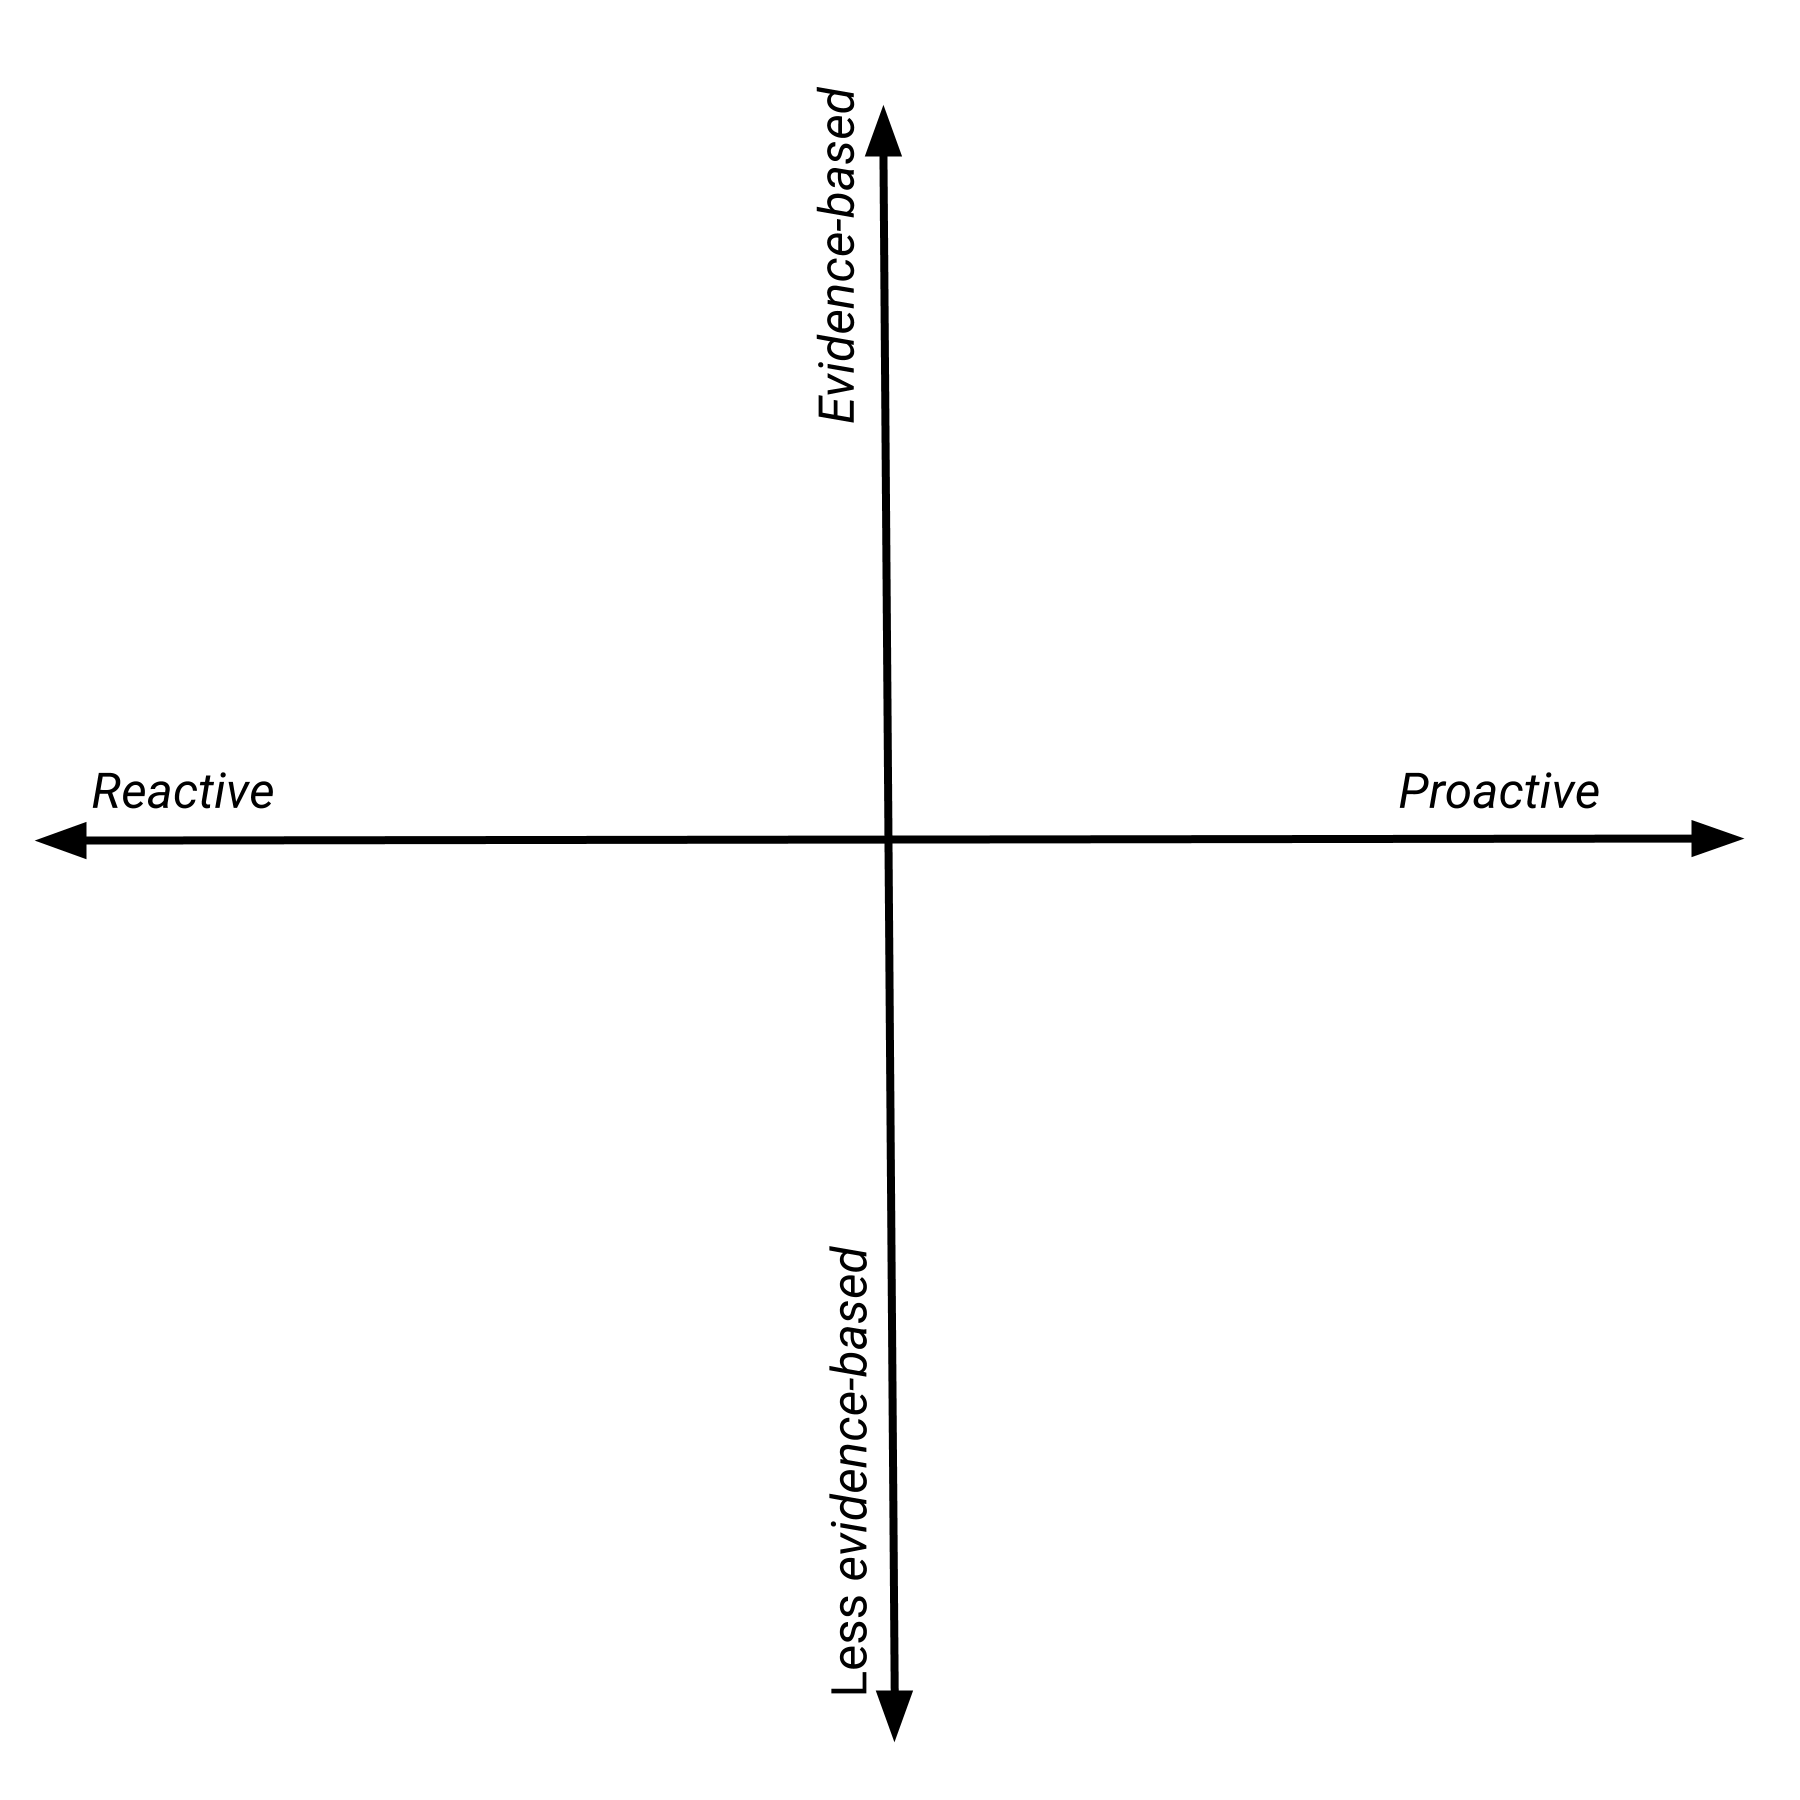
\includegraphics{files/CMEthics_context3.png}
\caption{Participants tended to vary according to how they approached
complementary medicines and how they approached evidence
\label{context3}}
\end{figure}

\subsubsection{Navigating practice in a retail
environment}\label{navigating-practice-in-a-retail-environment}

All participants discussed implications of the retail environment within
the context of fulfilling their professional obligations. Participants
who were pharmacy owners, in particular, recognised the impact of
complementary medicines on the financial bottom-line of the pharmacy.

\begin{quote}
I own a pharmacy \ldots{} I still work in the shop on a daily basis. So
I still come across on a daily basis having to chat to people about
this. But then I am also going to come at it from the side {[}that
complementary medicines{]} prop up half of the bank loan. So I guess we
are going to go both ways on this a little bit. (D5P7)
\end{quote}

Participants differed, however, in how they navigated practice in the
retail environment. Most participants sought to prioritize professional
obligations over financial considerations.

\begin{quote}
If a pharmacy's going to lose money for the sake of a sale, that isn't a
good enough reason for the sake of giving something out. We should
always be having a look at evidence-based treatments, \ldots{} (D4P5)
\end{quote}

These participants focused on ensuring appropriate practice within the
confines of financial constraints. Because participants differed in how
they viewed appropriate practice in the context of complementary
medicines, they also differed on the financial impost they were willing
to accept to fulfil the responsibilities outlined in the proposed
framework. This topic is discussed in detail below in relation to the
acceptability and feasibility of the framework.

\subsection{Context}\label{context}

Participants described how they approached complementary medicines in
day-to-day interactions with consumers as well as how they thought
pharmacists \emph{should} approach such interactions. They also
discussed what resources they had available to them to assist consumers
with complementary medicines as well as any barriers they experienced
when providing advice to consumers in relation to complementary
medicines. Topics frequently raised by participants in focus groups and
interviews were the role of naturopaths in community pharmacy, the
availability of resources on complementary medicines and the increasing
role of practitioner-only complementary medicine lines.
Practitioner-only lines have typically been sold by naturopaths working
in the pharmacy, but in recent years pharmacists have become more
actively involved in these sales. Most of these complementary medicines
are regulated in the same way as complementary medicines sold in the
front shop, but are marketed such that only certain practitioners can
sell the item (typically naturopaths and pharmacists). How participants
approached these topics was informed by the approach they took to
complementary medicines and their views regarding evidence. These views
are summarised in Figure~\ref{fig_context2}.

\begin{figure}
\centering
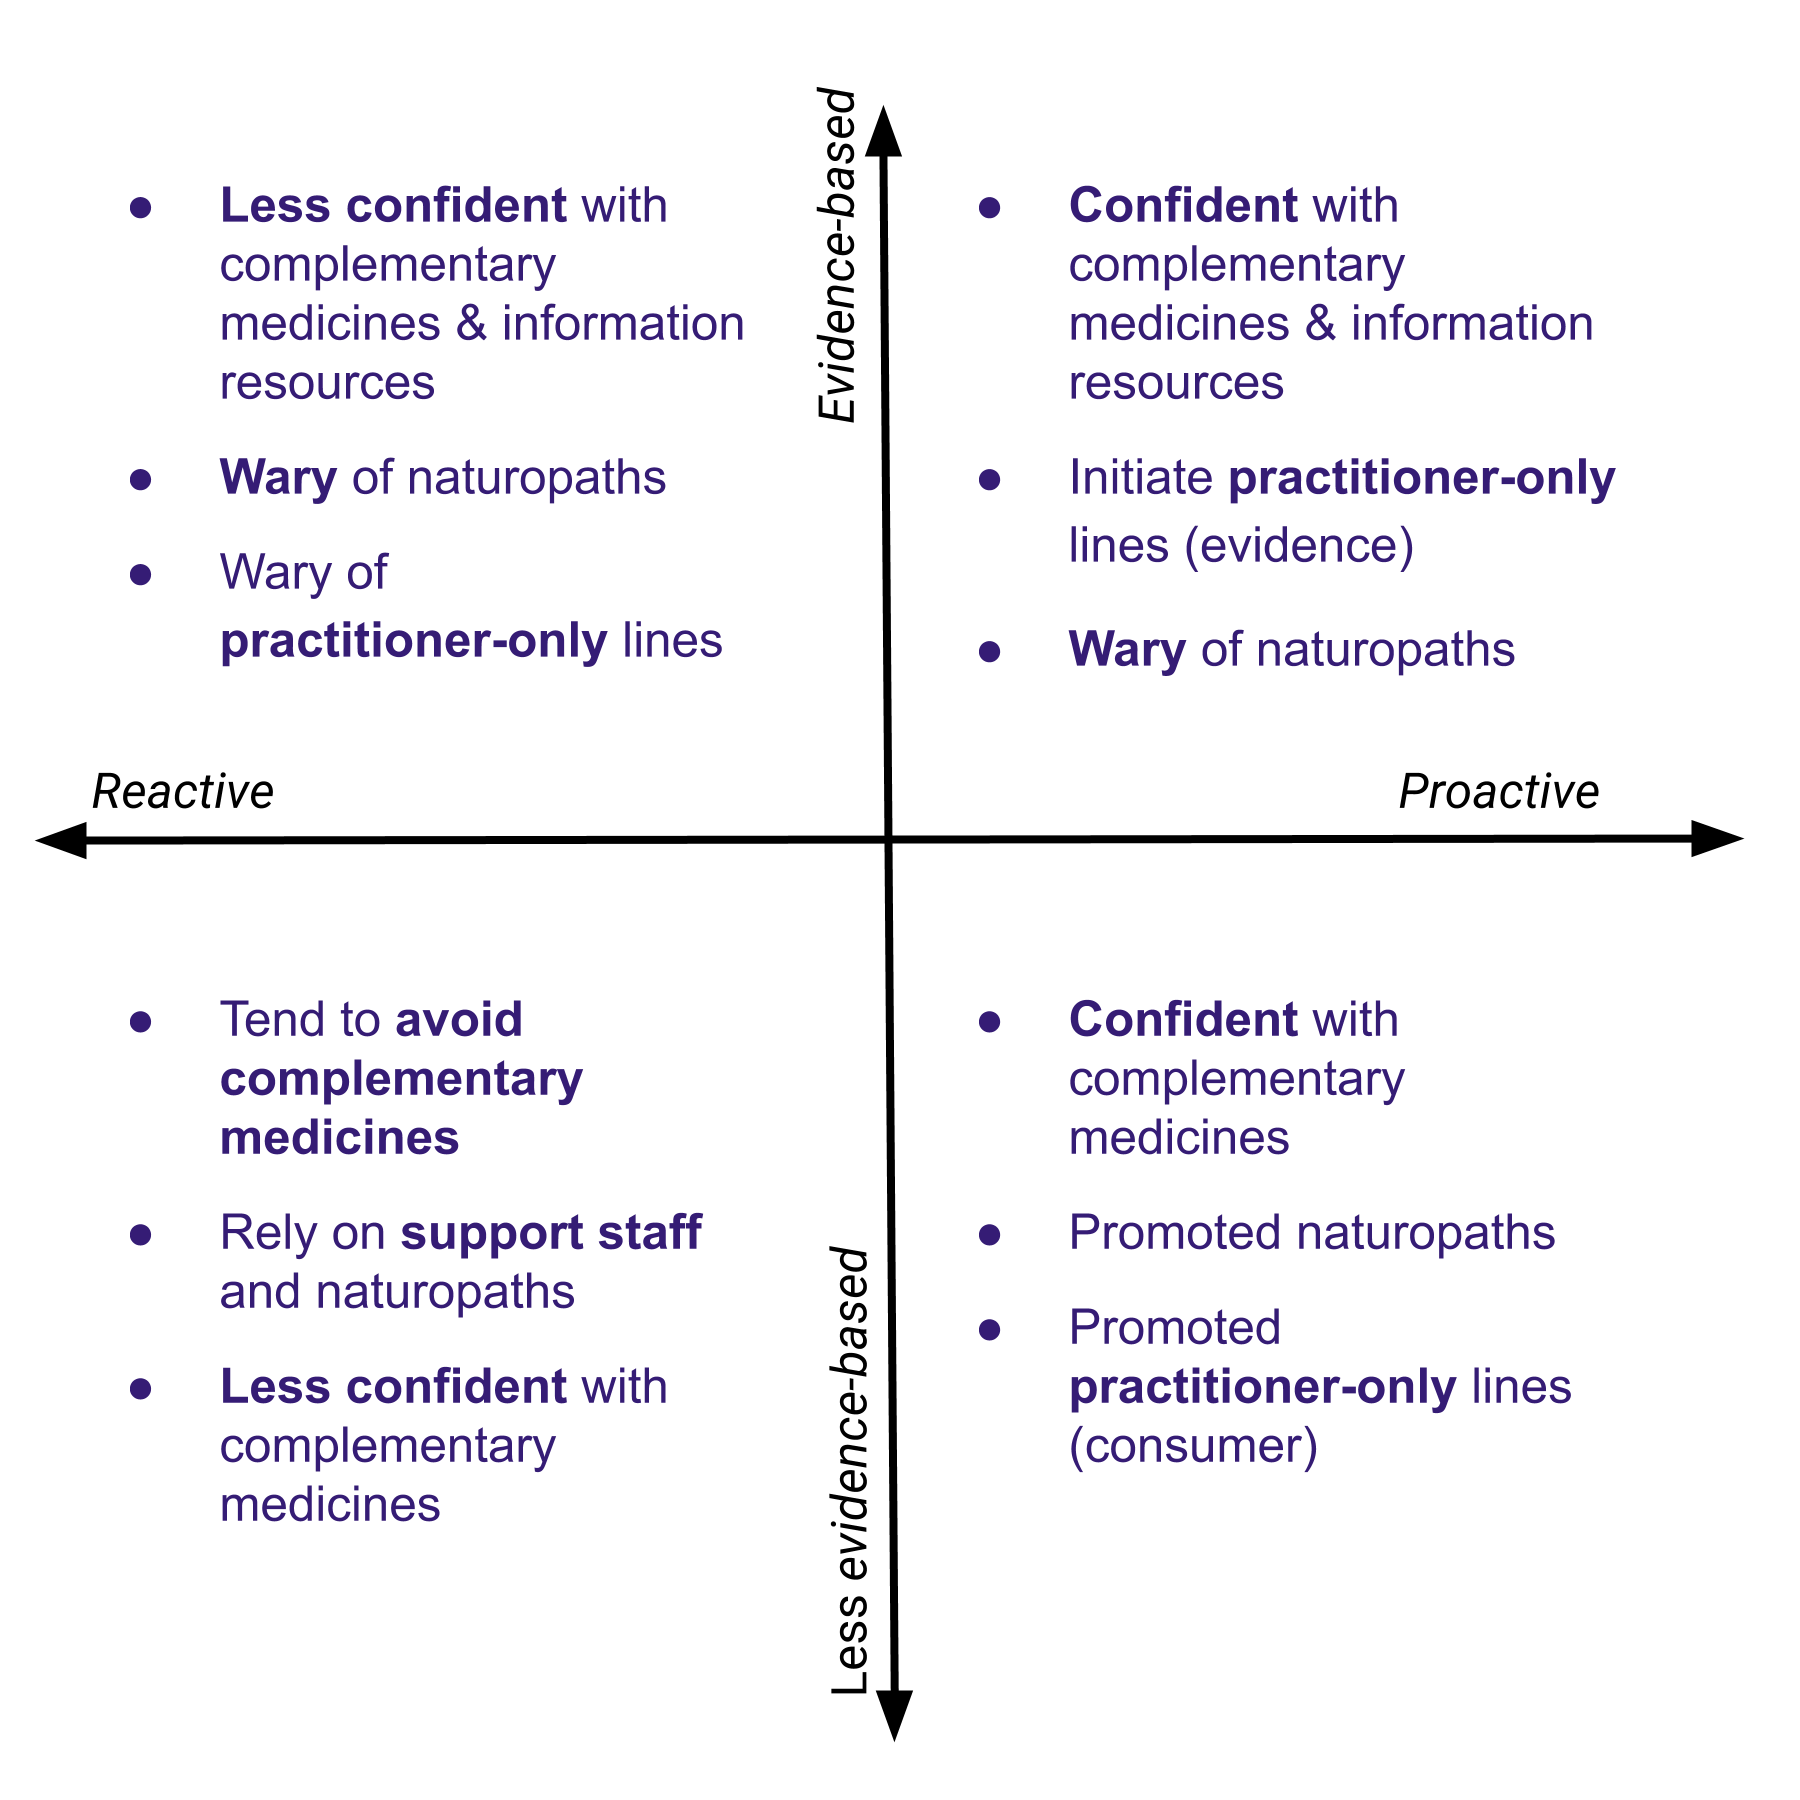
\includegraphics{files/CMEthics_context2.png}
\caption{How participants varied in relation to how they viewed the
context of providing advice on complementary medicines in community
pharmacy \label{fig_context2}}
\end{figure}

In brief, participants who were ``proactive'' and ``evidence-based''
tended to have access to and be confident users of information resources
on complementary medicines, actively recommend practitioner-only lines
and express concern regarding whether naturopaths provide evidence-based
advice. Participants who described their practice as evidence-based, but
took a more passive (reactive) approach to complementary medicines were
also wary about naturopaths, but were less likely to recommend
pracititioner-only lines and less likely to express confidence in
relation to information resources on complementary medicines.
Participants who were ``proactive'' and ``less evidence-based'' tended
to express confidence in relation to their knowledge and practice in
relation to complementary medicines as well as the knowledge and
practice of naturopaths. These participants actively recommended
practitioner-only lines. Participants who were ``less evidence-based''
and ``reactive'' in relation to complementary medicines tended to rely
on support staff and naturopaths to provide advice to consumer and
expressed a lack of confidence in relation to their knowledge and skills
in relation to complementary medicines.

\subsection{Acceptability of the framework}\label{acceptability}

Most participants felt the framework was acceptable: that it accurately
captured the responsibilities of pharmacists when selling complementary
medicines. Participants were more likely to express concern regarding
the feasibility of the framework. Participant views on the acceptability
and feasibility of the framework tended to be informed by how they
approached complementary medicines and how they approached evidence. The
other key determinant was how the participant navigated practice within
a retail environment. Participant views regarding the acceptability and
feasibility of the framework are summarised in Figure~\ref{accfeas}.

\begin{figure}
\centering
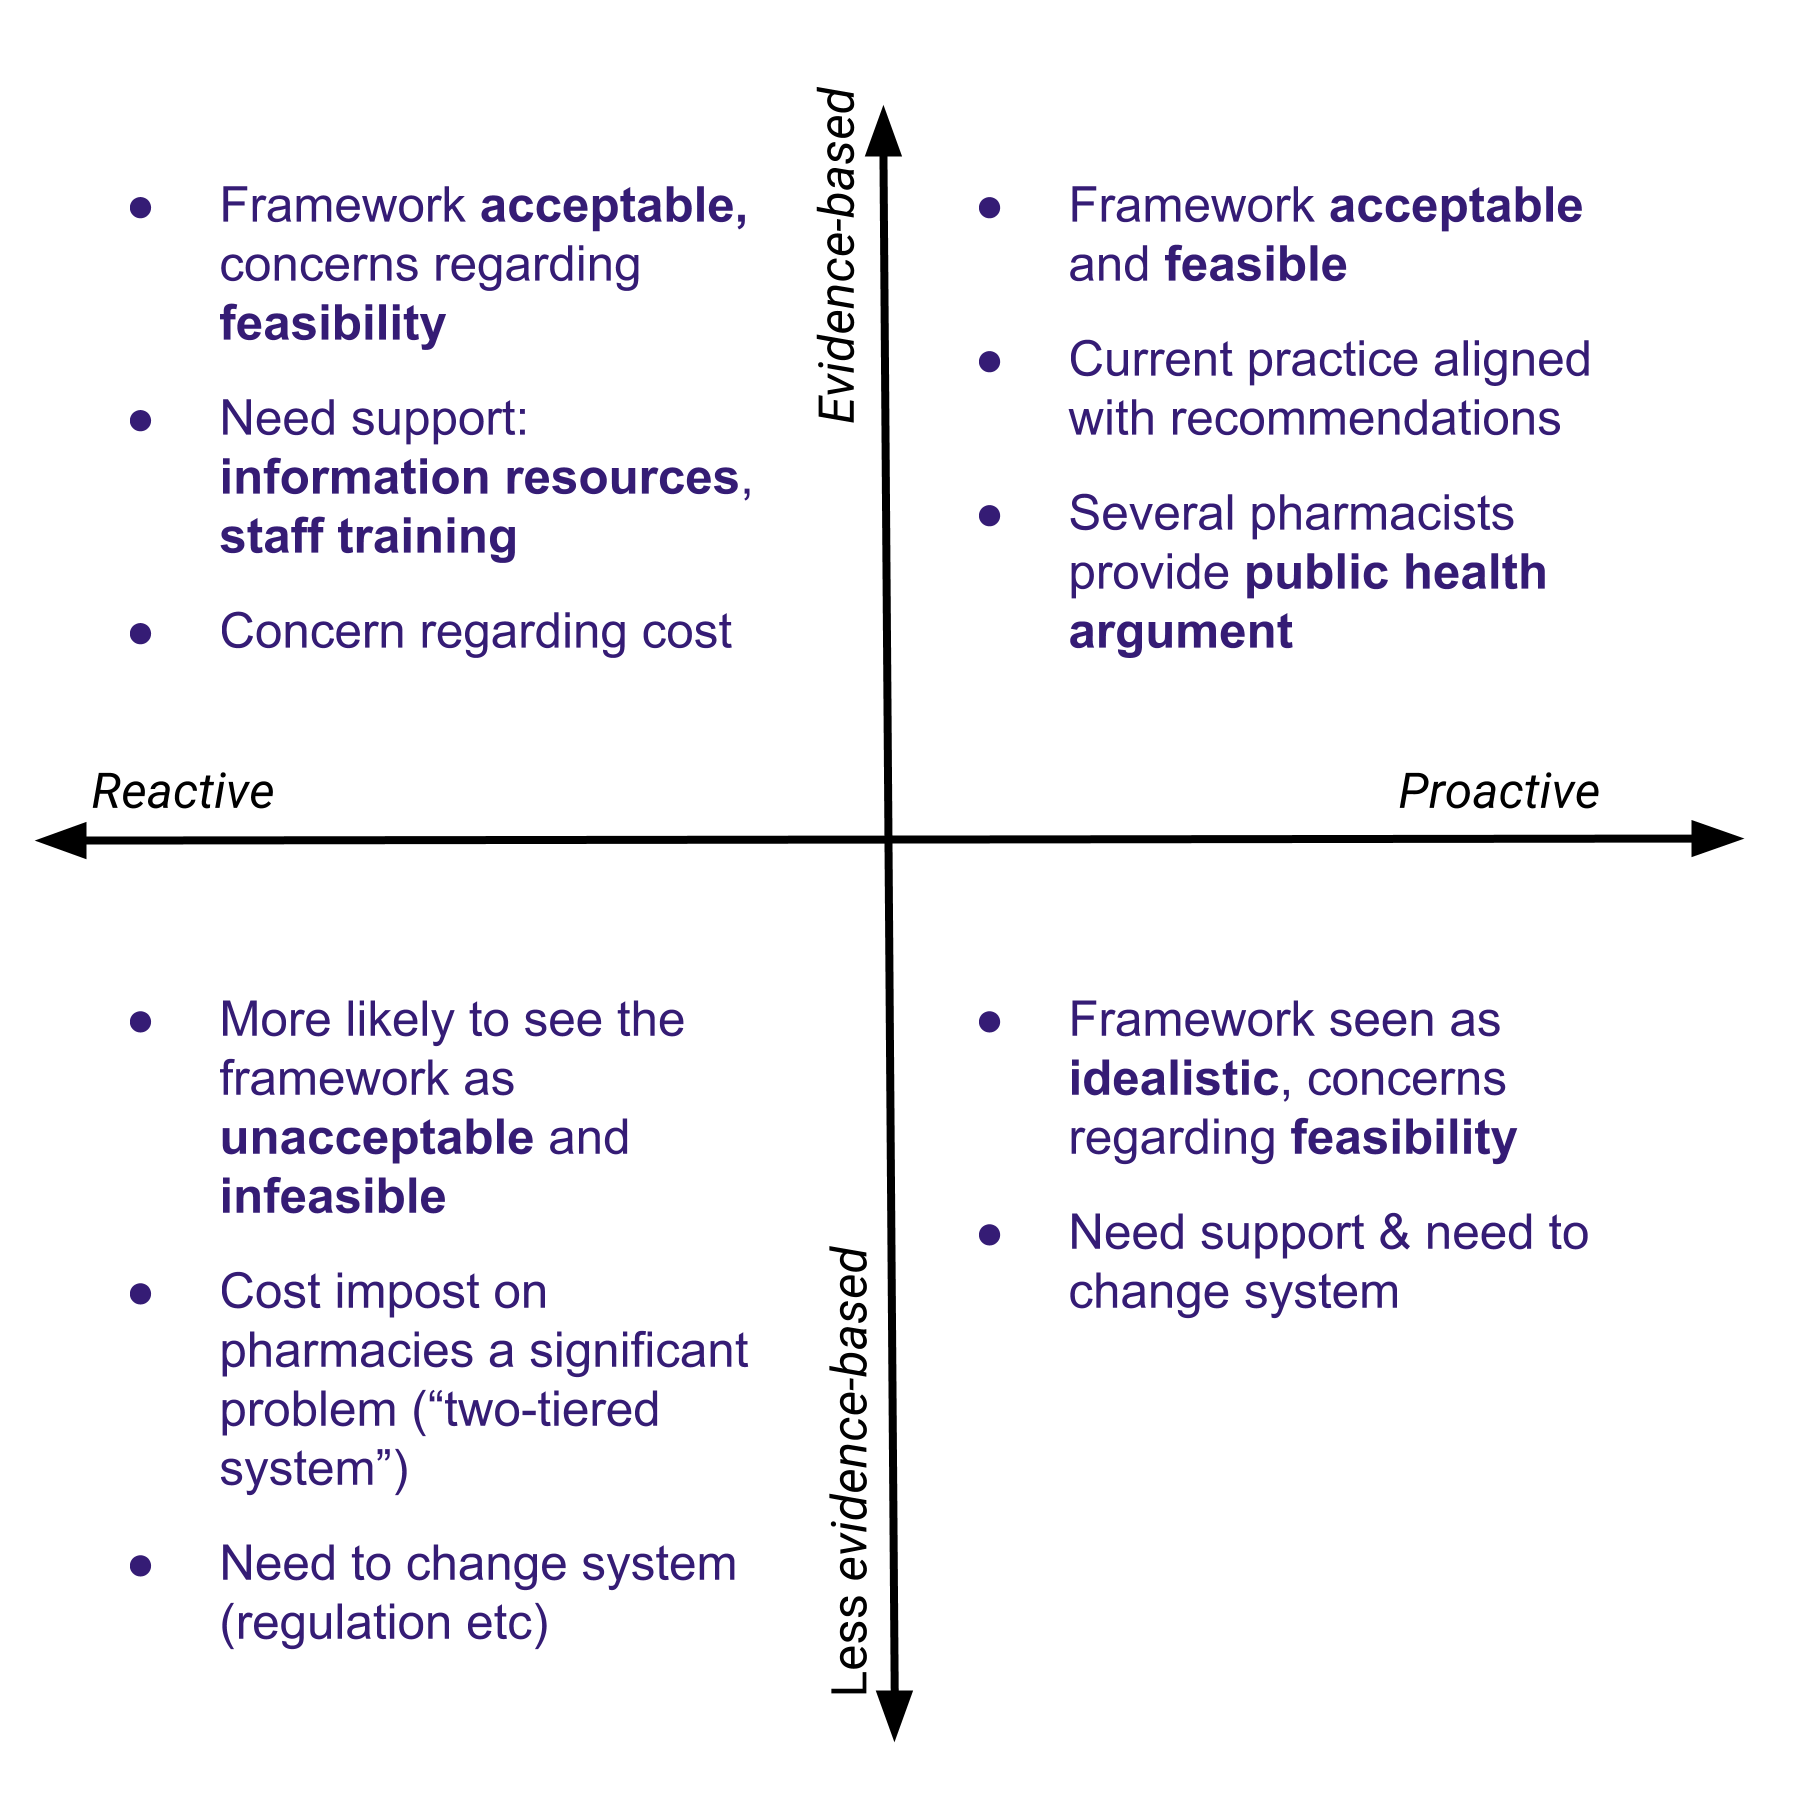
\includegraphics{files/CMEthics_accfeas.png}
\caption{How participants views on the acceptability and feasibility of
the framework different depending on how they approach complementary
medicines and evidence \label{accfeas}}
\end{figure}

Participants who were ``proactive'' \emph{and} ``evidence-based'' were
most strongly in favour of the proposed ethical framework. These
participants saw the framework as a being closely aligned with their
practice and commended the clear guidance the framework provided
regarding pharmacist responsibilities when selling complementary
medicines.

\begin{quote}
I think generally pharmacists are time poor and stressed and
overburdened, so anything that can make something more simplified and
streamlined with clear-cut expectations is useful. (D7P12)
\end{quote}

\begin{quote}
\ldots{}
\end{quote}

\begin{quote}
I would say {[}the framework is acceptable{]}, particularly with, yeah,
treating it along the lines of an S2 or an S3. So front-shop staff can
talk to the patients about it. If there's any further queries, the
pharmacist can be involved, but they don't automatically have to come
down and talk to them if it's not something that there's any questions
about. (D7P11)
\end{quote}

Several participants provided an argument along the lines of the public
health argument to support the sale of complementary medicines in
community pharmacies.

\begin{quote}
I think the reason that pharmacies should sell their complementary
medicine is not because there is a market. I think people, instead of
going to the health food store to get their {[}comple?{]} medicine, they
should come to the pharmacy because there is a better chance that the
pharmacies can find out if there's any interaction for people with some
actual medications. But I know most of my customers. I know exactly what
they are taking. If they come and someone on warfarin asks me for some
complementary medication, I just quickly before going and checking their
medical history, I know that that's not the right thing to give to the
person. But if that person goes to the health food store and buy it
there, there is no way that they can figure it out. So I think they
should be always at the pharmacy because people should think to go to
pharmacy to get their complementary medicine because that way they are
going to be protected and lots of trauma is going to be stopped. (D1P1)
\end{quote}

Two threats to acceptability were identified in the focus groups and
interviews. The primary perceived threat to the acceptability of the
framework was that it permits a ``two-tiered system'' for the sale of
complementary medicines. The framework identifies responsibilities for
pharmacies selling complementary medicines that are not expected of
other retailers. This point was raised in several focus groups and
interviews. The following quotes illustrate the back-and-forth between a
participant who argues the framework is not acceptable due to the
differential cost it imposes on community pharmacies and a second
participant who argues that part of being a pharmacist involves such
obligations.

\begin{quote}
I would say consumers mostly view {[}complementary medicines{]} as an
item of commerce. You buy them like you buy bread and milk, in some
instances, for some of them. So you've now imposed this cost on us
providing evidence, but in order to do that, we have to mark the product
up more. Then you've got this two-tiered system. (D5P7)
\end{quote}

\begin{quote}
I think that having the degree means that \ldots{} people come for a
higher level of service and understanding than what they can get in the
supermarket. And that's part of what differentiates us professionally.
And that's part of why it's still called a pharmacy and not a
supermarket. I'm comfortable that I would actually be probably more
comfortable practising where the TGA just says, ``Yes, that is safe to
take.'' And then the pharmacist makes the clinical judgement and says,
``Well, this may not be the best product for you.'' I think that that's
literally our goal. (D5P9)
\end{quote}

The second threat to the acceptability of the framework is a consequence
of the different approaches participants take to evidence-based
practice. The proposed framework assumes a shared understanding of what
is considered appropriate evidence for the efficacy of complementary
medicines. Participants who expressed an approach to evidence in
complementary medicines that was less evidence-based appear to hold a
different view. Accepting placebo effects as sufficient evidence of the
efficacy of complementary medicines and/or putting considerable weight
into the anecdotal experiences of others are approaches to evidence that
are incompatible with the framework. Similarly, for those who take the
view that placebo effects and anecdotal reports are sufficient evidence
for determining the efficacy of complementary medicine, the proposed
framework will be viewed as unacceptable.

The importance of taking this into account is illustrated in the
response some participants had to the guidance on complementary medicine
provided in the current \emph{Code of ethics for pharmacists}. For
example, some participants suggested that there were practising in
accordance with the guidance provided in the code of ethics on the basis
of the purported placebo effects of complementary medicines (see, for
example, the third quote in Section~\ref{approach-to-evidence}).
Determining appropriate evidence for assessing the effectiveness of
complementary medicines is complex and somewhat controversial. Some of
the considerations include the availability of well-conducted randomized
trials and the lack of impetus for such trials given they are not a
regulatory requirement. While it is not necessary (or feasible) to
resolve all of these issues for the purposes of the proposed framework,
it is necessary to identify some boundaries in relation to approaches to
evidence and complementary medicines. The findings of this study suggest
two such boundaries are the use of placebo effects and anecdotal reports
(in other consumers) as a justification for recommending complementary
medicines.

\subsection{Feasibility of the framework}\label{feasibility}

Participants tended to be more concerned about the feasibility of the
framework as opposed to its acceptability. The specific barriers that
participants identified, and the kinds of things that would enable
participants to overcome the barrier, depended on how participants
approached complementary medicines and evidence.

Participants who were ``evidence-based'' and ``proactive'' tended to see
the framework as both acceptable and feasible as presented. Participants
who were ``evidence based'' and ``reactive'' expressed concerns about
the feasibility of implementing the framework. These participants tended
to identify local, practical barriers and to identify areas of support
that would remedy these concerns. The two most consistently identified
barriers were the availability of (and confidence with) evidence-based
information resources on complementary medicines and staff training.
Some example quotes highlighting the importance of information resources
and training and some of the optimism participants expressed to
addressing these barriers:

\begin{quote}
Oh. I think it's a very nice framework in an ideal world, and if we are
provided with tools and training and the resources to train the staff, I
would be very happy to have that in the pharmacy. (D2P2)
\end{quote}

\begin{quote}
I feel like it would be really helpful if there was a better database to
look up interactions and all that type of thing because more often than
not, I have to call either the company or look into it really far to
make sure it doesn't interact. So maybe extra training in that area like
compulsory training, I guess. (D3P4)
\end{quote}

\begin{quote}
So I think, honestly, I would just be keen to try it out in the shop and
see how it actually works. But it's sort of one of those questions. If
you change the framework and require pharmacies to do something, some
sort of fundamental change in how we provide advice, would that open up
the space for a new database to actually provide some money so someone
would actually make it? Would that then mean that companies looking to
get their products into pharmacy would put more emphasis on evidence and
therefore training? So pharmacists wouldn't have to be doing these
trainings. You're going to get detailed by companies that are looking to
get the best, most evidence-based product into your stores. (D5P9)
\end{quote}

The absence of independent evidence-based training for pharmacy support
staff was identified as a barrier to implementing the framework. The
response to this is providing more opportunities for this kind of
training.

\begin{quote}
I've got 30 staff, and the idea that there could be more specialised
training for people that have that interest {[}in evidence-based
complementary medicines{]} and that could be another avenue for
non-pharmacists into pharmacy careers. Immediately, that's more
attractive than going to work at Woolies, where they just sell the stuff
en mass for profit?. How would that not be a good thing when we've
copped a lot of bad press about some pharmacists? So yeah, definitely. I
would be very interested to see if this framework allowed for more of
that. (D5P9)
\end{quote}

A number of participants identified an increased focus on
practitioner-only lines as one way to differentiate pharmacy services in
relation to complementary medicines while fulfilling the professional
obligations outlined in the framework.

\begin{quote}
Well, I feel like there should be, I guess, a shift away from the
front-shop selling. So just to distinguish pharmacy from the health food
store, so other things that people just see on TV or things that people
can buy without talking to a pharmacist or talking to someone that's
been trained in complementary medicines. So there's the idea of what
we've got, the pharmacy, with labelling it, even though it's not
necessarily a dangerous product, but just something that at least
requires a consult from the first go. Not every time but just from the
initial, first-selling to them so they know exactly why they're taking
it, rather than just they've been taking it for 10 years. And if we
said, ``Well, this is a better product, a better form of calcium or
whatever it might be,'' at least that way they can think of their
complementary medicines along the same lines as their regular
medications. So they still put some value on it, and they don't just
look for the cheapest option or the most convenient, necessarily, but
something that they get more value out of. (D7P11)
\end{quote}

Participants who described their practice in a way that was less
evidence based tended to agree with the barriers and facilitators
identified above as well as express additional concerns regarding the
feasibility of implementing the framework. Participants who were
``proactive'' and ``less evidence-based'' tended to see the framework as
acceptable though idealistic, and suggest that it could only be
implemented if there were significant system changes made to support the
framework. Participants who were ``reactive'' and ``less
evidence-based'' were more likely to view the framework as both
unacceptable and infeasible. These participants had significant concerns
about cost implications. The system changes that each of these groups of
participants suggested were similar. Suggestions included ensuring all
pharmacies implemented the framework in a similar way (perhaps taking a
regulatory approach to assessing compliance with the framework) and
making changes to the way the complementary medicines were regulated
such that there were tighter restrictions on the availability of
complementary medicines.

\begin{quote}
\ldots{}{[}G{]}etting all the pharmacies on the same page. If you've got
pharmacies that are run by corporations and banner groups that are more
for-profit versus small community pharmacies that are trying to provide
a service. You've got to have these frameworks that are enforceable,
maybe through QCPP or a PBS listing, and make sure that everyone does
the same things and stocks the same products and doesn't stock the same
products based on evidence. (D7P12)
\end{quote}

\begin{quote}
The next thing, I think, would be TGA. If they're approving it, but then
it's not evidence based, then consumers will get confused because they
would say, ``Oh, but then it's approved by TGA, so it must be all right
or evidence based.'' (D10P17)
\end{quote}

\begin{quote}
Why should it be up to us as pharmacists? Why shouldn't the TGA---when
it goes to them in the first place to be approved, why is it even
getting to us? Why are we required to make the decision? Why haven't TGA
done their job? (D5P7)
\end{quote}

\section{Discussion \&
recommendations}\label{discussion-recommendations}

The \emph{Framework for pharmacist responsibilities when selling
complementary medicines} provides specific guidance to pharmacists on
fulfilling their responsibilities when selling complementary medicines.
The framework seeks to address current gaps in the professional and
academic literature with regard to the availability of specific
professional guidance supported by an explicit theoretical approach. It
balances pharmacist responsibilities to providing evidence-based health
care, to promote positive health outcomes and to respect consumer health
beliefs and preferences. The study findings suggest that the proposed
framework will be acceptable to most pharmacists and is feasible to
implement with some targeted support.

The focus groups provided a way to explore group norms in relation to
professional responsibilities when selling complementary medicines as
well as to discuss and explore proposed ethical framework. The strengths
of the study include the variation present in the demographic details of
the participants, and the features of the qualitative methods that
permit an in-depth examination of how the participants approached
complementary medicines and the framework. Some of the limitations of
the study arise due to the methods used. Different methods with a larger
representative sample of pharmacists would be required to estimate the
prevalence of different approaches to complementary medicines in
Australian community pharmacy (e.g. ``evidence-based'', ``proactive'',
etc). Further, the study did not include consumers or pharmacy support
staff. While not specifically in relation to proposed ethical framework,
the perspectives of these groups have been explored elsewhere
\autocite{Iyer2016a}.

Recommendations:

\begin{itemize}
\tightlist
\item
  Move participants towards the upper right quadrant (``EBP'',
  ``proactive'')
\item
  Support regarding information resources
\item
  Training: for pharmacists and for pharmacy support staff

  \begin{itemize}
  \tightlist
  \item
    Pharmacists: use current skills (not become naturopaths)
  \item
    Pharmacy support staff: independent evidence-based training
  \end{itemize}
\end{itemize}

\printbibliography[title=References]

\end{document}